\documentclass[10pt]{article}
\usepackage{graphicx, subfigure}

%functions
\setlength{\parindent}{0in}

\newcommand{\code}[1]{\texttt{#1}}

\newcommand{\fig}[3]{
	\begin{figure}[!ht]
	\centering
	\includegraphics[scale=#3]{img/#1}
	%\includegraphics[width=420px]{img/#1}
	\caption{#2}
	\label{fig:#1}
	\end{figure}
}
\newcommand{\fignocaption}[3]{
	\begin{figure}[!ht]
	\centering
	\includegraphics[scale=#3]{img/#1}
	\label{fig:#1}
	\end{figure}
}

\newcommand{\figw}[3]{
	\begin{figure}[!ht]
	\centering
	\includegraphics[width=#3]{img/#1}
	\caption{#2}
	\label{fig:#1}
	\end{figure}
}

\newcommand{\figs}[6]{
	\begin{figure}[!ht]
	\centering
	\subfigure[#5]{
		\includegraphics[width=14cm]{img/#2}
		\label{fig:#2}
	}
	\subfigure[#6]{
		\includegraphics[width=14cm]{img/#3}
		\label{fig:#3}
	}
	\caption{#4}
	\label{fig:#1}
	\end{figure}
}
\newcommand{\figsSmall}[6]{
	\begin{figure}[!ht]
	\centering
	\subfigure[#5]{
		% width=14cm
		\includegraphics[width=5cm]{img/#2}
		\label{fig:#2}
	}
	\subfigure[#6]{
		% width=14cm
		\includegraphics[width=5cm]{img/#3}
		\label{fig:#3}
	}
	\caption{#4}
	\label{fig:#1}
	\end{figure}
}


\title{\sc Optimizing 3D models from 2D images}

\author{T. Kostelijk\\mailtjerk@gmail.com}

%\date{December 16, 2010}

\begin{document}

\maketitle
\begin{abstract}
Here comes the abstract
\end{abstract}

% todo
% new structure of paper
% explain food nodde
% explain algo's
% smooth intensity gradient
% pictures
% write introductions
% explain motivation behind decisions
% explain what is new or what is unique
% todo background section?



\section{Introduction}
 \subsection{Related work}
 \subsection{FIT3D toolbox}
 \subsection{Organization of this thesis}

\section{Projective Geometry}
	% get inspiration and/or copy from Isaacs paper 
	% introduce K
	% introduce 2d to 3d projection

\section{Skyline detection}
 \subsection{Introduction}

The sky and the earth are separated by a skyline in images. The detection of this skyline
has proven to be very succesful computer vision application in a wide range of
domains. In this domain it is used to provide a countour of a building. This
contour is in a next step used to refine a 3D model of this building.\\
The organisation of this chapter is as follows.  First related work on skyline
detection is discussed, then a new algorithm of the skyline algorithm is
described and finally some results are presented.\\
% It is interesting to denote that the skyline detector a stand alone method and
% can be optimized individually without any knowledge of the other parts of the
% project.
 \subsection{Related work}
A lot of related work on skyline detection is done and it is used in a wide
range of domains. $[1]$ yields a good introduction of different skyline
detection techniques, these are listed below.

\subsubsection{Cloud detection for Mars Exploration Rovers (MER)}
Mars Exploration Rovers (MER) are used to detect clouds and dust devils on Mars.
In [1] their approach is to first identify the sky (equivalentl, the skyline)
and then determine if there are clouds in the region segmented as sky.
%todo why or why not interesting for this thesis?

\subsubsection{Horizon detection for Unmaned Air Vehicles (UAV)}
In this domain, the horizon detector for UAVs can take advantage of the high
altitude of the vehicle and therefor the horizon can be approximated to be a
straigt line.  This turns the detection problem into a line-fitting problem.
Ofcourse this work is not applicable for detecting a building countour as the
straight line assumption doesn't work. But it needs to be mentioned that from this
idea some inspiration on line fitting is done because the building countour has
straight line segments.

\subsubsection{Planetary Rover localisation}
In [9] they use the skyline detection in planetary rovers, their approach is to
combine the detected skyline with a given map of the landscape (hills, roads) to
detect its current location. 
The advantage of their technique is the simplicity and effectiveness of the
algorithm which makes it suitable for this project.  A big drawback is that it
is geared toward speed over extremely high accuracy because it is 
interactive system where an operator refines the skyline.

As mentioned in the introduction, in this project we use the skyline to extract
the building contour to eventually update a 3D model which is a brand new
purpose of skyline detection.  There is no user interaction present, and the
accuracy is a matter of high importance.  This makes it different from existing
skyline techniques and caution should be taken by using existing algorithms.
From the related work the Planetary Rover localisation [9] seemed to fit most on
this project.  Therefor method [9] is used, but as a basis, and a custom
algorithm with higher accuracy is developed. This is explained in the next
section.

%talk about assumptions
%there are always this assumptions??
%but what can we (not) assume?
%Furthermore we can assume that some straight lines 

\textit{todo why?}
 \subsection{The Algorithm}
 \subsubsection{The original algorithm}
 %TODO lezen: Map-based localization using the panoramic horizon
The skyline detection algorithm as described in $[9]$ works as follows:
The frames are first preprocessed by converting them to Gaussian smoothed images.
The skyline of a frame is then detected by analysing the the image columns
seperately.
The smoothed intensity gradient is calculated from top to bottom. This is done
by taking the derivative of the gaussian smoothed image.
The system takes the first pixel with gradient higher then a threshold to be
classified as a skyline element.  This is done for every column in the image.
The result is a set of coordinates of length $W$,
where $W$ is the width of the image, that represent the skyline.

Taking the smoothed intensity gradient is the most basic method of edge
detection and has the disadvantage that is is not robust to more vague
edges. This is not surprising as it its purpose was a interactive system where the
user refines the result. It is clear that an optimization is needed.

  \subsubsection{The optimization}
 % page 15/16
 % idea for future work:
 % adaptive thresholding wrt average intensity!
The column based approach seem te be very useful and is therefor unchanged. 
The effectiveness of the algorithm is totally depended of the method of edge
detection and the preprocessing of the images. 
The original algorithm uses the smoothed intensity gradient as a way of
detecting edges. This is a very basic method and more sophisticated edge
detection algorithms are present.\\
To select a proper edge detector, a practical study is done on the different
Matlab build in edge detection techniques. The output of the different edge
detection techniques was studied and the Sobel edge detector came with the most
promising results. The Sobel edge detector outputs a binary image, therefor the column inlier
threshold method is replaced by finding the first white pixel. This is as the
original algorithm done from top to bottom for every column in the image.
\\ 
To make the algorithm more precise, two preprocessing
steps are introduced. First the contrast of the image is increased, this makes
sharp edges stand out more.  Secondly the image undertakes a Gaussian blur,
this removes a large part of the noise.

The system now has several parameters which has to be set manually by the user:
\begin{itemize}
\item contrast,
% officialy i don't do this contrast thing
\item intensity (window size) of Gaussian blur,
\item Sobel edge detector threshold,
\end{itemize}
\textit{Should I write down what parameter values I used or is this of too much
detail}

If the user introduces a new dataset these parameters needs to be changed
as the image quality and lightning condition are probably different.
%(Automatic parameter estimation based on the image would be interesting future
%work but lies without the scope of this research.)

 \subsection{Results}%%%%%%%%%%%%%%%%%%%%%%%%%%%%%%%%%%%%%%%%%%%%%%%%%%%%
The system assumes that the first sharp edge (seen from top to bottom) is
always the skyline/building edge. This gives raise to some outliers, for 
for example a streetlight or a tree. These outliers are removed as described in
the next section.  

The Skyline detector without outlier removal has an accuracy of 80 \% 

Some results from the Floriande dataset:
%TODO quote Isaac here
%\fig{outputSkylineIm3\_1.jpg}{this is a test}{this is an other test}


%TODO results uitleggen wat is wat, whuut whuuut whuuut (southpark stijl)
\begin{figure}[!ht]
\centering
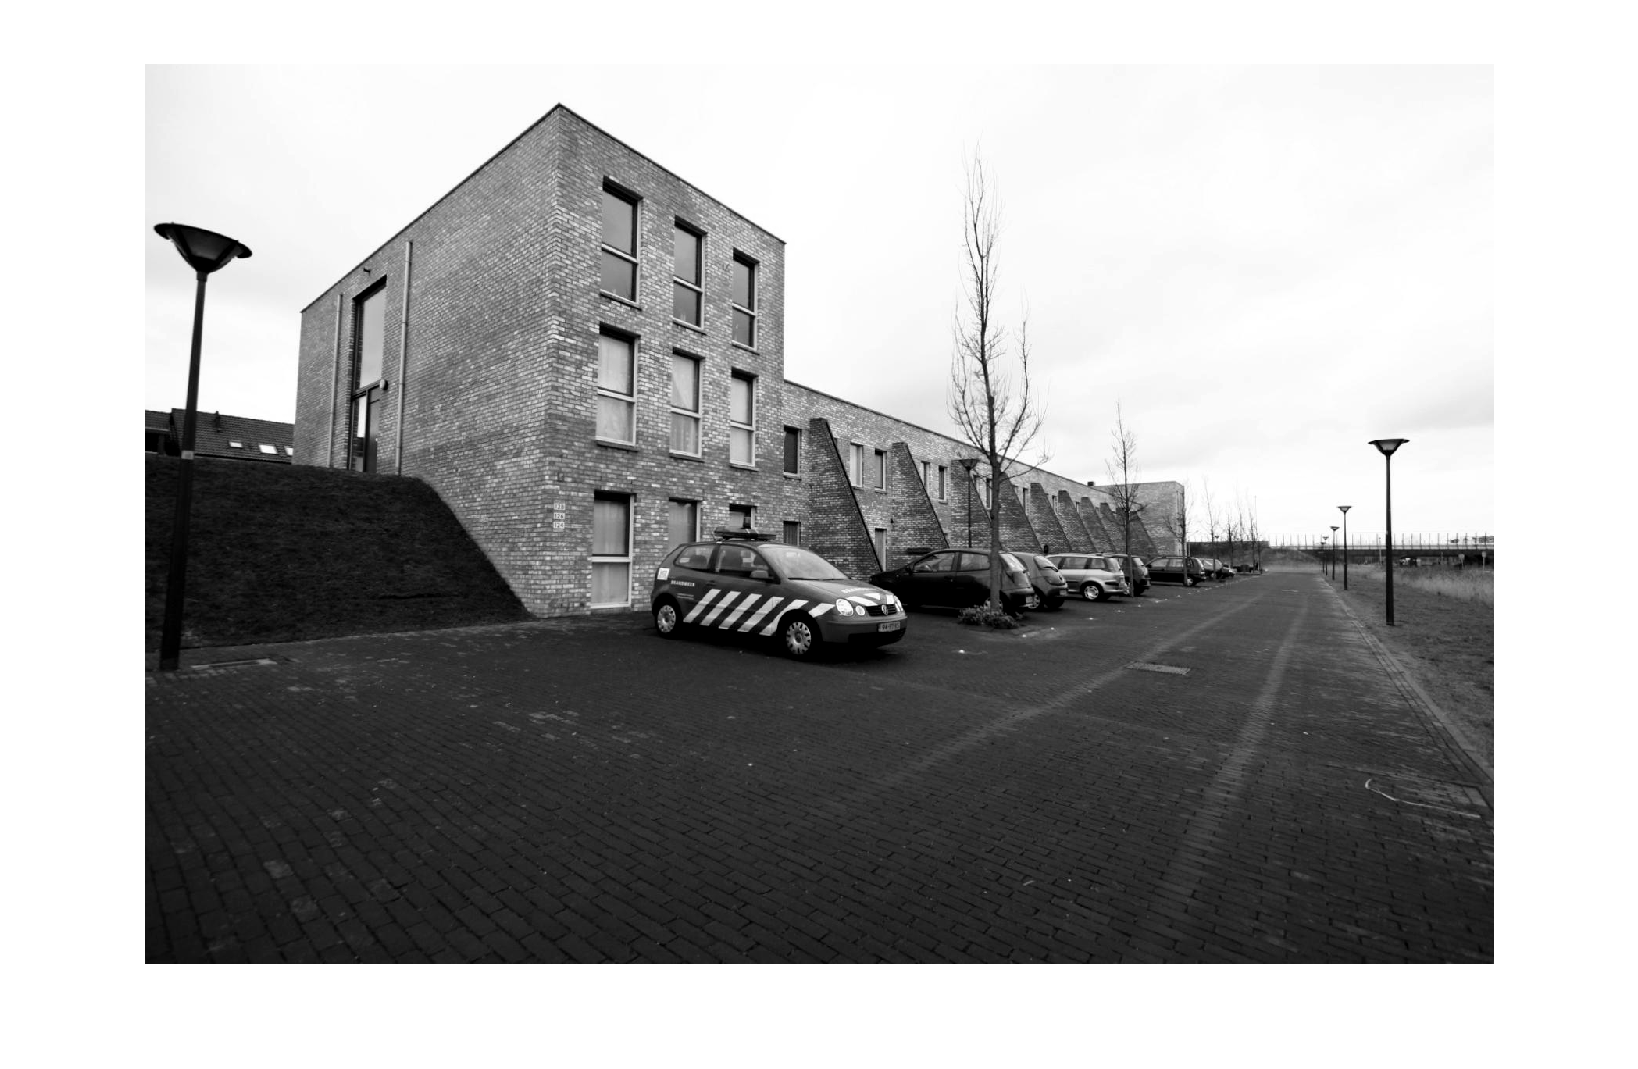
\includegraphics[scale=0.5]{img/outputSkylineIm3-1.eps}
\caption{abc}
\end{figure}

\textit{ TODO Results images}
\textit{ TODO make UML scheme skyline -> 3d -> etc.}
\\

\section{Skyline projection}
 \subsection{Introduction}
The retrieved skyline is used to update a sparse 3D model of the building.
This section describes how the skyline of the 2D images are used to get the 3D contour of the building. 

\textit{TODO convert to algorithm or method }
 
\subsection{Project to 3D space}
\textit{ TODO situation scheme}
Every 2D pixel of an input image presents a 3D point in space. No
information is known about the distance from the 3D point to the camera. What
is known is de 2D location of the pixel, this reduces the possible points in 3D
space to an infinite line.  This line is known and spanned by two 
coordinates:\\ 
\begin{itemize}
	\item The camera center %(camera centers are annotated for every image)
	\item $K'p$, where $K$ is the Calibration matrix of the camera and $p$ is the homogeneous pixel coordinate.
\end{itemize}

\textit{ TODO why K'p,I don't remember the theory behind it and can't find it in Isaac's paper }
For every skyline pixel a line spanned by the above two coordinates is derived.

\subsection{Intersect with building}
The line is reduced to a point in 3D by intersecting it with a rough indication
of the building. This point is used to update the 3D model.\\
To create a rough indication of the building a top-view photograph of the
building is used together with an estimate of the height of the building.\\ 
In order to refine this sparse 3D model we need to know which skyline part belongs to which part of
the 3D model. This is done as follows.\\
The building is first divided into different walls.  Every wall of the building spans a plane. 
As described in the previous section every part (pixel) of the skyline presents an infinite line in 3D.
Intersections are calculated between these infinite lines and the planes of the building walls.\\
\textit{ Isaac, should I put a intersection formula down here or is this trivial?}\\
Because the lines and the planes are both infinite and they have a very low change
of being exactly parallel, the algorithm returns $w$ intersections for every
skylinepixel (where $w$ is the number of walls).\\
Next challenge is to reduce the number of intersection for every skylinepixel
to one. In other words, to determine the wall that has the largest probability of
being responsible for that pixel. This is ofcourse needed to update the 3D
model at the right place.

\subsection{Find most likely wall}
\subsubsection{When is a wall responsible?}
Lets define the intersection between the projected skylinepixel line and the
plane of the wall as intersection point $isp$. And the wall sides as ${w1, w2,
w3, w4 \in W}$. And $d$ as a distance measure which is explained later on.\\ If
we assume that a certain wall was responsible for that pixel, the intersection
(i.e. projected pixel) must lie either\\

\textbf{(1)} Somewhere on the wall 
\\
or
\\
\textbf{(2)} On a small distance $d$ from that wall
(1) is calculated by testing if the pixel lies inside the polygonal
representation of the wall. This is done using the Matlabs buildin in-polygon
algorithm. If this test succeeds we consider $d$ to be 0.\\

(2) Note that this is treated as an inlier because the 3D model is sparse and the height of
the building is estimated. It is calculated as follows: \\
First the distances from $isp$ to four wall sides are calculated.
For every wall the minimum distance is stored.\\
$min_{w\in W} d(isp, w)$\\
This is done for every wall. The wall with the smallest distance is the one that most likely presents the pixel.\\
$arg min_{W \in Walls} ( min_{w\in W} d(isp, w) )$\\
\textit{ do I write this down correctly?}

%threshold..

If there are two (or even more) walls that are classified equally well to
present the pixel (that is if they succeed the in-polygon or have exactly the
same $d$ value) then the nearest wall is selected. The nearest wall is
calculated by taking the wall with the smallest distance from the $isp$ to the
camera center.
\textit{ formula here? or: trivial?}\\
How this intersection point - wall distance $d$ is calculated is explained in
the next section.

\subsubsection{Calculate the intersection point - wall distance}
A wall consists of four corner points. The corner-point pairs that are on a
side of the wall connect line segments, there are four line segments. These
line segments span infinite lines.\\

The intersection point ($isp$) is projected orthogonally on these four lines, a
projected $isp$ is called $isp_{proj}$.
\textit{ todo image?}
\textit{ todo projection formula?}

If $isp$ is close to a wallside, $e(isp, isp_{proj})$ (where $e$ is defined as
the Euclidean distance) is small.  But this doesn't mean that if
$e(isp,isp_{proj})$ is small $isp$ is always close to the wall. In fact there are
some candidates that happen to have a very small $d(isp, isp_{proj})$ but in fact
lie far away from the wall. This is because $isp$ is projected to an infinite
line spanned by the wallside and could be projected far next to the wallside.
\textit{ An example can be seen in figure:}
\textit{ TODO Figure}
Because of this artefact, it is not robust to calculate the perpendicular
projection distance.  Instead $d$ is calculated differently if $isp_{proj}$
doesn't lie on the wallside.  In this case the Euclidean distance between
$isp_{proj}$ and the closest corner-point of the wallside is returned.

Formally:
Let $c1,c2,c3,c4 \in Cornerpoints$ be the corners of a wall.\\
Let $between(a,b,c)$ be a function that returns true if a lies between b and c.\\
if $between(isp_{proj}, c1, c2)$\\
$d = e(isp, isp_{proj})$\\
otherwise\\
$d = min_{c \in Cornerpoints} e(isp, c)$\\
\\
\textit{TODO nice latex code with large \} sign}\\


\subsubsection{Appendix?: Determine whether $isp_{proj}$ lies on or next to a wallsegment}


% todo ref: http://softsurfer.com/Archive/algorithm_0102/algorithm_0102.htm

% todo P -> $P$
To determine whether the $isp_{proj}$ lies on or next to a wallsegment the
projection calculation is skipped and $isp$ is used instead together with a
computational cheap trick.\\

%todo
%\fig{shortestProjection.gif}{TODO caption}{1}

\textit{ todo insert http://softsurfer.com/Archive/algorithm\_0102/Pic\_segment.gif here}\\
First consider Figure ?? , the angles between the segment P0P1 and the vectors P0P and P1P
from the segment endpoints to P. If both angles are equal to or less than
$90^{\circ}$ then the $isp_{proj}$ wil be on the line segment P0 P1.  If not,
the $isp_{proj}$ lies to the left or to the right of segment P according to
whether one of the angles is acute or obtuse.  The angles are acute or obtuse
if the dot product of the vectors involved are respectively positive or
	negative.\\
To summarize: determining in which region the $isp_{proj}$ lies is boiled down to
two dot product calculations with the advantage that the actual projection
calculation can be skipped.
%Again this result determines if the distance should be computed to one of the
%corner points P0 or P1, or as the perpendicular distance to the line L (the
%wallside) itself.


\textit{Todo come back on outlier removal}
\subsection{Results}

\section{Update 3D model}


\section{References}
\begin{itemize}
\item $[1]$ Castano, Automatic detection of dust devils and clouds on Mars.
\item $[9]$ Cozman, Outdoor visual position estimation for planetary rovers.
\end{itemize}

\end{document}


